\documentclass[a4paper,10pt]{scrbook}

\usepackage{geometry}
\geometry{verbose,a4paper,tmargin=2.5cm,bmargin=2.5cm,lmargin=2.5cm,rmargin=2cm}

\usepackage[pdftex]{graphicx}

%\usepackage{ifthen}



% Macht beim fett schreiben auch das Mathe-Zeug fett
%
\newcommand{\allbf}[1]{\textbf{\boldmath#1\unboldmath}}

% FANCY CAPTION
% \caption[#1]{\textbf{#1}#1}
\newcommand{\mycaption}[2]{\caption[#1]{\textbf{\boldmath#1\unboldmath} #2}}







%%%
%%% Now you can use \ifcolor as follows
%%% \ifcolor
%%%    Text parsed by PDFLaTeX
%%% \else
%%%    Text parsed if PDFLaTeX is not used
%%% \fi
%%% 
\newif\ifcolor\colortrue



%
%   COLOR
%
%
\usepackage{color}
\definecolor{brightred}{rgb}{1,0.9,0.9}
\definecolor{brightgreen}{rgb}{0.9,1,0.9}
\definecolor{brightblue}{rgb}{0.95,0.95,1}
\definecolor{brightyellow}{rgb}{1,1,0.85}

\definecolor{lightred}{rgb}{1,0.75,0.75}
\definecolor{lightgreen}{rgb}{0.75,1,0.75}
\definecolor{lightblue}{rgb}{0.75,0.75,1}
\definecolor{lightyellow}{rgb}{1,1,0.75}

\definecolor{red}{rgb}{1,0,0}
\definecolor{green}{rgb}{0,1,0}
\definecolor{blue}{rgb}{0,0,1}

\definecolor{darkred}{rgb}{.7,0,0}
\definecolor{darkgreen}{rgb}{0,.7,0}
\definecolor{darkblue}{rgb}{0,0,.7}

\definecolor{white}{rgb}{1,1,1}
\definecolor{lightgray}{rgb}{0.95,0.95,0.95}
\definecolor{gray}{rgb}{0.5,0.5,0.5}
\definecolor{black}{rgb}{0,0,0}

\definecolor{marker}{rgb}{0.9,0.9,0.9}
\definecolor{urgent}{rgb}{1,0,0}
\definecolor{discreeturgent}{rgb}{1,0.5,0.5}
\definecolor{discreetcomment}{rgb}{0.25,0.9,0.25}
\definecolor{checked}{rgb}{0,.7,0}



%\newif\ifshowtasks\showtaskstrue
\newif\ifshowtasks\showtaskstrue
\newcommand{\task}[1]{\ifshowtasks\textcolor{discreeturgent}{~#1~}\else\fi}
\newcommand{\comment}[1]{\ifshowtasks\textcolor{discreetcomment}{~#1~}\else\fi}
\newcommand{\drain}[1]{}

%
%    LISTINGS
% \begin{lstlisting}[float,caption=A floating example]
%    for i:=maxint to 0 do
%    begin
%      { do nothing }
%    end;
%    Write(’Case insensitive ’);
%    WritE(’Pascal keywords.’);
% \end{lstlisting}
%
% for referencing line numbers use (*@\label{comment}@*)  inside the lstlistings enviroment
\usepackage{listings}
\ifcolor
          \lstset{							% general command to set parameter(s)
               escapeinside={(*@}{@*)},
               xrightmargin=0.5cm,					% for centering
               xleftmargin=1.5cm,					% .. \textwidth shrinks after the first time, which is stupid
               framexleftmargin=20pt,					% for having the numbers beneath the h rules
               framexrightmargin=0pt,
               framextopmargin=2ex,					% draw good looking space between the lines
               framexbottommargin=2ex,					%... and the listing
               frame=single,						% h rules top and bottom
               language=C,
               tabsize=4,
               numbers=left,
               numberstyle=\footnotesize, 
               numbersep=8pt,
               basicstyle=\ttfamily\scriptsize, 		% print whole listing small
               breaklines=true,
               keywordstyle=\color{black}\bfseries,		% underlined bold black keywords
               identifierstyle=,				% nothing happens
               commentstyle=\color{darkblue}\itshape,		% white comments
               stringstyle=\ttfamily, 				% typewriter type for strings
               morekeywords=[2]{and,or,not},
               emph={wichtiges,zeug},				% additional keywords
               emphstyle=\underbar,
               showstringspaces=false} 				% no special string spaces
\else
          \lstset{						% general command to set parameter(s)
               escapeinside={(*@}{@*)},
               xrightmargin=0.5cm,				% for centering
               xleftmargin=1.5cm,
               framexleftmargin=20pt,				% for having the numbers beneath the h rules
               framexrightmargin=0pt,
               framextopmargin=2ex,				% draw good looking space between the lines
               framexbottommargin=2ex,				%... and the listing
               frame=single,					% h rules top and bottom
               language=C,
               tabsize=4,
               numbers=left,
               numberstyle=\footnotesize, 
               numbersep=8pt,
               basicstyle=\scriptsize\ttfamily,			% print whole listing small
               breaklines=true,
               keywordstyle=\color{black}\bfseries,		% underlined bold black keywords
               identifierstyle=,									% nothing happens
               commentstyle=\color{black}\itshape,			% white comments
               stringstyle=\ttfamily, 							% typewriter type for strings
               morekeywords=[2]{and,or,not},
               emph={wichtiges,zeug},								% additional keywords
               emphstyle=\underbar,
               showstringspaces=false} 						% no special string spaces
\fi

%
\usepackage[labelfont={bf},font=small]{caption,subfig} 
% justification=raggedright,format=hang,labelfont={bf},font=small
% justification=justified,singlelinecheck=false

%
%    HYPERREF
%
%    (depends on z_layout_settings color)
%
% NO HANDLING YET FOR NOT PDF!!!
\ifcolor
  \usepackage[pdftex,
            colorlinks=true, linkcolor=blue, urlcolor=blue, citecolor=blue,
            raiselinks=true,
            bookmarks=false,
            bookmarksopenlevel=1,
            bookmarksopen=true,
            bookmarksnumbered=true,
            hyperindex=true,
            plainpages=false,% correct hyperlinks
            pdfpagelabels=true%,% view TeX pagenumber in PDF reader
            %pdfborder={0 0 0.5}
            ]{hyperref} % erzeuge Hyperlinks z.B. für pdflatex
\else
  \usepackage[pdftex,
            colorlinks=true, linkcolor=black, urlcolor=black, citecolor=black,
            raiselinks=true,
            bookmarks=false,
            bookmarksopenlevel=1,
            bookmarksopen=true,
            bookmarksnumbered=true,
            hyperindex=true,
            plainpages=false,% correct hyperlinks
            pdfpagelabels=true%,% view TeX pagenumber in PDF reader
            %pdfborder={0 0 0.5}
            ]{hyperref} % erzeuge Hyperlinks z.B. für pdflatex
\fi





\newcommand{\lstsetCPP}{%
\ifcolor%
\lstset{
	escapeinside={//(@*}{*@)},
	language=C++,
	frame=single,
	numbers=left,
	backgroundcolor=\color{brightblue}
	}%
\else%
\lstset{
	escapeinside={//(@*}{*@)},
	language=C++,
	frame=single,
	numbers=none,
	backgroundcolor=\color{white}
	}%
\fi%
}

\newcommand{\lstsetARCHEDXML}{%
\lstset{
	escapeinside={<!--(@*}{*@)-->},
	language=XML,
	frame=single,
	numbers=left,
	backgroundcolor=\color{lightyellow}
	}%
}

\newcommand{\lstsetJUSTXML}{%
\lstset{
	escapeinside={<!--(@*}{*@)-->},  % <!--(*@\label{comment}@*)-->
	language=XML,
	frame=single,
	numbers=left,
	backgroundcolor=\color{brightyellow}
	}%
}


\newcommand{\lstsetKSH}{%
\lstset{
	escapeinside={(@*}{*@)},
	language=ksh,
	frame=single,
	numbers=none,
	backgroundcolor=\color{lightgray}
	}%
}

% Sometimes latex just won't accept a line break.
% With this command you can do it anyway! HAR HAR HAR
\newcommand{\forcelinebreak}{
%\vspace{\bigskipamount}
\hspace*{\fill} \\
} 


\usepackage{framed}                                %for shaded and framed paragraphs
\usepackage{textcomp}                              %for various symbols, e.g. Registered Mark
%
\def\efill{\hfill\nopagebreak}%
\hyphenation{Nordu-Grid}
\setlength{\parindent}{0cm}
\setlength{\FrameRule}{1pt}
\setlength{\FrameSep}{8pt}
\addtolength{\parskip}{5pt}
\renewcommand{\thefootnote}{\fnsymbol{footnote}}
\renewcommand{\arraystretch}{1.3}
\newcommand{\dothis}{\colorbox{shadecolor}}
\newcommand{\globus}{Globus Toolkit\textsuperscript{\textregistered}~2~}
\newcommand{\GT}{Globus Toolkit\textsuperscript{\textregistered}}
\newcommand{\ngdl}{\url{http://ftp.nordugrid.org/download}~}
\definecolor{shadecolor}{rgb}{1,1,0.6}
\definecolor{salmon}{rgb}{1,0.9,1}
\definecolor{bordeaux}{rgb}{0.75,0.,0.}
\definecolor{cyan}{rgb}{0,1,1}
%
%----- DON'T CHANGE HEADER MATTER

\hypersetup{
  pdfauthor = {},
  pdftitle = {Webservices},
  pdfsubject = {Paper subject},
  pdfkeywords = {HED,ARC},
  pdfcreator = {PDFLaTeX with hyperref package},
  pdfproducer = {PDFLaTeX}
}

\begin{document}


%
% You can use KILE to browse through these tex-files.
% Just lookout for the tutorial.kilepr in the root directory.
%

\def\today{\number\day/\number\month/\number\year}

\begin{titlepage}

\begin{tabular}{rl}
\resizebox*{3cm}{!}{\includegraphics{ng-logo.png}}
&\parbox[b]{2cm}{\textbf \it {\hspace*{-1.5cm}NORDUGRID\vspace*{0.5cm}}}
\end{tabular}

\hrulefill

{\raggedleft NORDUGRID-D2.5-2 ???\par}

{\raggedleft \today\par}

\vspace*{2cm}

%%%%---- The title ----
{\centering \textsc{\Large Dynamic Runtime Environment Installation with Janitor}
\\\vspace{1cm} \normalsize\textcolor{discreeturgent}{The Janitor and this document with it is under continuous development. Your comments and suggestions are appreciated.} % DELETE ONLY THAT LINE!!!
\Large \par}
\vspace*{0.5cm}

%%%%---- A subtitle, if necessary ----
%{\centering \textit{\large Paper subtitle}\large \par}

\vspace*{1.5cm}
%%%%---- A list of authors ----
    {\centering \large Michael Glodek, Daniel Bayer,  Steffen M\"oller\footnote{moeller@inb.uni-luebeck.de} \par}

%%%%---- An abstract - if style is article ----
%\begin{abstract}
%The abstract
%\end{abstract}
\end{titlepage}

\tableofcontents                          %Comment if use article style
\newpage
%\chapter{Preface}
%\section{Introduction}                    %Use Sections for articles
%\label{sec:intro}

\sloppy

../../../manuals/janitor/tex_introduction/introduction.tex
\chapter{The time webservice}


The first implementation of a Web Service which will be presented in this tutorial realises a simple time service.
In case the service receives a request, it will respond with a string containing the systemtime.
For simplicity the service will not parse the request but always return the current time.
In the following subsections the C++ implementation first the service and than the client will be developed.


\section{Service}

In Arc-1 the services are implementated as plugins such that they can easily be included by modifiying the HED configuration file as it was to be seen in Listing~\ref{lst:arched_arcecho_xml}.
The Listing~\ref{lst:time_arched_cpp}.shows the implementation of the time service plugin.
The proper class definition is defined in the corresponding header file which isn't shown here.
The key element for each plugin is the struct PluginDescriptor named PLUGINS\_TABLE\_NAME, see line\ref{lst_code:time_cpp_ptn}. 
%The struct defines basic entities of the service and provides a pointer to the method which is able to create an instance of the time service plugin. 
Within the struct a unique plugin name, the type of the plugin, its version and the pointer to the function which returns the time service instance has to be defined.
The function which returns the pointer to an instance of the service needs to have the PluginArgument as a parameter. 
The actual Time Web Service is implemented within the namespace ArcService. The constructor can be found in line~\ref{lst_code:time_cpp_constructor}, the deconstructor in line~\ref{lst_code:time_cpp_deconstructor} and the method required by the inherited class \textit{Service} file in line~\ref{lst_code:time_cpp_process}. For the Time service is very simple, only the function process needs to be implemented. It gets the incoming and the outgoing message as references and returns a class representing the status the service achieved. 
\lstsetCPP
\lstinputlisting
	[
	label=lst:time_arched_cpp,
	caption={[C++ implementation of the time service. Filename: timeservice.cpp]
	\textbf{C++ implementation of the time service. Filename: timeservice.cpp}}
	]
{../src/services/timeservice/timeservice.cpp}
The service first determines the current time and than creates a SOAP message using the object \textit{PayloadSOAP} on line~\ref{lst_code:time_cpp_process_payloadSOAP}. The class \textit{PayloadSOAP} is able to create a XML message which is conform to the SOAP protocol (The apperance of the generated request and response will be discussed later). I case of the presented time service the payload consists out of two elements nested into one another. The element \textit{text} holds the element child which again holds the string containing the current time.
Within the line~\ref{lst_code:time_cpp_process_message_payload} the payload is passed to the message. 
The message processing is now completed and the function returns its success status on line~\ref{lst_code:time_cpp_return}.
The source code has to be compiled to a dynamic library named \textit{libtimeservice.so}.\\


After the service has been implemented and compiled, it needs to be loaded into the HED. A suitable HED configuration file is to be seen in Listing~\ref{lst:time_arched_xml}. 
\lstsetARCHEDXML
\begin{program}
\lstinputlisting
	[
	label=lst:time_arched_xml,
	caption={[HED configuration for the time service. Filename: arched\_timeservice.xml]
	\textbf{HED configuration for the time service. Filename: arched\_timeservice.xml}}
	]
{../src/services/timeservice/arched_timeservice.xml}
\end{program}
A new path element has been introduced into the element \textit{ModuleMananger}, line~\ref{lst_code:arched_time_moduleManager}. It assigns the location to the compliled dynamic library. 
On line~\ref{lst_code:arched_time_plugin} the library is explict mentioned to be loaded.
Another important change has been done within the \textit{Plexer} element in line~\ref{lst_code:arched_time_plexer_next}. A rule has been introduced which redirects the request to the Time Web Service, if the path of URL is \textit{time}.\\


To run the service again the arched command shown in~\ref{lst:arched_timeservice_ksh} has to be used.
\lstsetKSH
\begin{program}
\begin{lstlisting}[
label=lst:arched_timeservice_ksh,
caption={[Transformation in eine uniforme konzentrische Verteilung.]
         \textbf{Transformation in eine uniforme konzentrische Verteilung.\textcolor{white}{hmf}}}]
$ arched -c arched_timeservice.xml && echo Daemon started || echo Daemon start failed
Daemon started
\end{lstlisting}
\end{program}



\section{Client}

\task{\#ifdef HAVE\_CONFIG\_H\#include <config.h>\#endif - habe ich entfernt... macht keinen Sinn, da keine weiteren Macros im Source Code enthalten sind... oder?}
In the next step a simple client needs to be implemented whose task is to interprete the returned message of the client.
The client needs to have the same protocol stack as the daemon but in contrast to it, it does not need the ability to be loaded as a plugin. As one will see, the creation of this protocol stack on client side is very simple.
The source code of the client consists primarily of the main function and is to be seen in Listing~\ref{lst:time_client_cpp}.
In line~\ref{lst_code:time_client_cpp_logger} the logger is initialized and redirected to the standard error stream.
For the components of the protocol stack are likewise loaded dynamically, one need to specify the installation directory in line~\ref{lst_code:time_client_cpp_init} too.
\task{remark in \textbf{introduction}, what the plexer is for. In our case: to have several services running on one port!!!!!!!!}
The URL of the service is defined in line~\ref{lst_code:time_client_cpp_url}. It fits to the HED configuration file which was shown in Listing~\ref{lst:time_arched_xml}. The daemon is listing on port 60000 and is running on the localhost. The service itself uses HTTP and can be reached by using the path \textit{time}.
Line~\ref{lst_code:time_client_cpp_config} loads the standard config file which is usually almost empty. As a result, no additional security procedures will later be linked into the client sided stack. The protocol stack is created in line~\ref{lst_code:time_client_cpp_client}. Thanks to the URL the information for the configuration can be completed.
The constructor of the class \textit{ClientSOAP} creates a SOAP client which uses HTTP, addresses the port 60000 on localhost. If i.e. HTTPS would have been used, the stack would have been extended by a TLS layer.
Now the client stack is ready, one can create a request to the service. In line~\ref{lst_code:time_client_cpp_message_reqeust} a message which corresponds to the Listing~\ref{lst:time_client_request} is created. The message gets processed by the command in line~\ref{lst_code:time_client_cpp_message_response}. If everything was fine, the message will finally be send to the standard out in line~\ref{lst_code:time_client_cpp_message_answer}.

\lstsetCPP
\lstinputlisting
	[
	label=lst:time_client_cpp,
	caption={[HED configuration file for the Arc intern echo service. Filename: arcecho\_no\_ssl.xml]
	\textbf{HED configuration file for the Arc intern echo service. Filename: arcecho\_no\_ssl.xml\textcolor{white}{hmf}}}
	]
{../src/clients/timeclient/timeclient.cpp}





The data is enveloped by an element called \textit{Envelope} .. See german wiki

\lstsetJUSTXML
\begin{minipage}[t]{\textwidth}
\begin{lstlisting}[
label=lst:time_client_request,
caption={[Transformation in eine uniforme konzentrische Verteilung.]
         \textbf{Transformation in eine uniforme konzentrische Verteilung.\textcolor{white}{hmf}}}]
<soap-env:Envelope xmlns:time="urn:time" xmlns:soap-enc="http://schemas.xmlsoap.org/soap/encoding/" xmlns:soap-env="http://schemas.xmlsoap.org/soap/envelope/" xmlns:xsd="http://www.w3.org/2001/XMLSchema" xmlns:xsi="http://www.w3.org/2001/XMLSchema-instance">
  <soap-env:Body>
    <time>
      <timeRequest></timeRequest>
    </time>
  </soap-env:Body>
</soap-env:Envelope>
\end{lstlisting}
\end{minipage}


\lstsetJUSTXML
\begin{minipage}[t]{\textwidth}
\begin{lstlisting}[
label=lst:time_client_response,
caption={[Transformation in eine uniforme konzentrische Verteilung.]
         \textbf{Transformation in eine uniforme konzentrische Verteilung.\textcolor{white}{hmf}}}]
<soap-env:Envelope xmlns:soap-enc="http://schemas.xmlsoap.org/soap/encoding/" xmlns:soap-env="http://schemas.xmlsoap.org/soap/envelope/" xmlns:xsd="http://www.w3.org/2001/XMLSchema" xmlns:xsi="http://www.w3.org/2001/XMLSchema-instance">
  <soap-env:Body>
    <time>
      <timeResponse>Wed Feb 18 11:20:30 2009</timeResponse>
    </time>
  </soap-env:Body>
</soap-env:Envelope>
\end{lstlisting}
\end{minipage}




\lstsetKSH
\begin{minipage}[t]{\textwidth}
\begin{lstlisting}[
label=st:time_client_ksh,
caption={[Transformation in eine uniforme konzentrische Verteilung.]
         \textbf{Transformation in eine uniforme konzentrische Verteilung.\textcolor{white}{hmf}}}]
$ ./timeclient
Wed Feb 18 11:20:30 2009
\end{lstlisting}
\end{minipage}













\chapter{The echo service}

The next service which will be presented is the echo service. It simply returns the received message back to the client.
Depending on the operation requested by the client, the letters of the message will be reordered reverse or not.
The goal of this chapter is to offer a deeper knowledge in message processing. Furthermore the \textit{WSDL} (Web Services Description Language) shall be introduced along with this example.

\section{Web Services Description Language}

Web Services are often reachable for a large set of users in order to easily access complex information. In many cases the Web Service are capable to replace HTML pages i.e. access to databases like Pubmed or the NLM catalog.
% http://www.ncbi.nlm.nih.gov/entrez/query/static/esoap_help.html
In contrary to HTML the interfaces of the data are well defined and easier to find for machines. bla...
Due to that reason, the way to access the web service has to be defined in an own language: \textit{WSDL} (Web Services Description Language).
WSDL is a meta language which determines the structure of the messages along with its permitted elements, the accepted operations, the supported protocols and the address to reach the service. 
The WSDL for the echo service which shall be implemented in this chapter is to be seen in Listing~\ref{lst:echo_wsdl}. There are five main elements to describe a service:
\begin{itemize}
	\item \textbf{Types} --- Definition of the data types used by the messages, line~\ref{lst_code:echo_wsdl_types}.
	\item \textbf{Message} --- Assignments which data types are representing a message, line~\ref{lst_code:echo_wsdl_message1} and \ref{lst_code:echo_wsdl_message2}.
	\item \textbf{Port type} --- \parbox[t]{13cm}{Assignment of the interface: One-way (input), request-response (input, output), solicit-response (input, output, fault), notification (output). The request-response interface is used in line~\ref{lst_code:echo_wsdl_portType}.}
	\item \textbf{Binding} --- Defines the concret protocol and data format used for the message transmission, line~\ref{lst_code:echo_wsdl_binding}.
	\item \textbf{Service} --- Specifies the address to bind a service, line~\ref{lst_code:echo_wsdl_service}.
\end{itemize}
%\textcolor{white}{newline}
\lstsetJUSTXML
\lstinputlisting
	[
	label=lst:echo_wsdl,
	caption={[WSDL file describing the echo service. Filename: echo.wsdl]
	\textbf{HWSDL file describing the echo service. Filename: echo.wsdl}}
	]
{../src/services/echoservice/echo.wsdl}


More information about WSDL may be found at \href{http://www.w3.org/TR/wsdl}{http://www.w3.org/TR/wsdl}.

% a valid service request and the  


% WSDL ist eine Metasprache, mit deren Hilfe die angebotenen Funktionen, Daten, Datentypen und Austauschprotokolle eines Web Service beschrieben werden können. Es werden im Wesentlichen die Operationen definiert, die von außen zugänglich sind, sowie die Parameter und Rückgabewerte dieser Operationen. Im Einzelnen beinhaltet ein WSDL-Dokument funktionelle Angaben zu:

%    * der Schnittstelle
%    * Zugangsprotokoll und Details zum Deployment
%    * Alle notwendigen Informationen zum Zugriff auf den Service, in maschinenlesbarem Format

%Nicht enthalten sind hingegen:

%    * Quality-of-Service-Informationen
%    * Taxonomien/Ontologien zur semantischen Einordnung des Services

\section{Service}

The service defined by the WSDL file in the previous section shall now be implemented. The source code of the C++ file is shown in Listing~\ref{lst:echo_service_cpp}. Again the header file will be set aside for it contains to much redundant information.

\lstinputlisting
	[
	label=lst:echo_service_cpp,
	caption={[C++ implementation of the echo service. Filename: echoservice.cpp]
	\textbf{C++ implementation of the echo service. Filename: echoservice.cpp}}
	]
{../src/services/echoservice/echoservice.cpp}


\lstsetARCHEDXML

\lstinputlisting
	[
	label=lst:arcecho_arched_xml, float=htb,
	caption={[HED configuration file for the Arc intern echo service. Filename: arcecho\_no\_ssl.xml]
	\textbf{HED configuration file for the Arc intern echo service. Filename: arcecho\_no\_ssl.xml\textcolor{white}{hmf}}}
	]
{../src/services/echoservice/arched_echoservice.xml}





\lstsetKSH
\begin{lstlisting}[
label=lst:invokation_arched_timeservice,float=htb,
caption={[Transformation in eine uniforme konzentrische Verteilung.]
         \textbf{Transformation in eine uniforme konzentrische Verteilung.\textcolor{white}{hmf}}}]
$ arched -c arched_echoservice.xml  && echo jo ||echo n
\end{lstlisting}



\section{Client}


\lstsetCPP
\lstinputlisting
	[
	label=lst:arcecho_arched_xml,
	caption={[HED configuration file for the Arc intern echo service. Filename: arcecho\_no\_ssl.xml]
	\textbf{HED configuration file for the Arc intern echo service. Filename: arcecho\_no\_ssl.xml\textcolor{white}{hmf}}}
	]
{../src/clients/echoclient/echoclient.cpp}

\lstsetCPP




\lstsetKSH
\begin{lstlisting}[
label=lst:invokation_arched_timeservice, float=htb,
caption={[Transformation in eine uniforme konzentrische Verteilung.]
         \textbf{Transformation in eine uniforme konzentrische Verteilung.\textcolor{white}{hmf}}}]
$ ./echoclient http://localhost:60000/echo ordinary text_to_be_transmitted
[ text_to_be_transmitted ]
$ ./echoclient http://localhost:60000/echo reverse text_to_be_transmitted
[ dettimsnart_eb_ot_txet ]
\end{lstlisting}





\lstsetJUSTXML
\begin{lstlisting}[
label=lst:timeservice_cpp_source, float=htb,
caption={[Transformation in eine uniforme konzentrische Verteilung.]
         \textbf{Transformation in eine uniforme konzentrische Verteilung.\textcolor{white}{hmf}}}]
<soap-env:Envelope xmlns:echo="urn:echo" xmlns:soap-enc="http://schemas.xmlsoap.org/soap/encoding/" xmlns:soap-env="http://schemas.xmlsoap.org/soap/envelope/" xmlns:xsd="http://www.w3.org/2001/XMLSchema" xmlns:xsi="http://www.w3.org/2001/XMLSchema-instance">
  <soap-env:Body>
    <echo:echoRequest>
      <echo:say operation="reverse">text_to_be_transmitted</echo:say>
    </echo:echoRequest>
  </soap-env:Body>
</soap-env:Envelope>
\end{lstlisting}



\lstsetJUSTXML
\begin{lstlisting}[
label=lst:timeservice_cpp_source, float=htb,
caption={[Transformation in eine uniforme konzentrische Verteilung.]
         \textbf{Transformation in eine uniforme konzentrische Verteilung.\textcolor{white}{hmf}}}]
<soap-env:Envelope xmlns:echo="urn:echo" xmlns:soap-enc="http://schemas.xmlsoap.org/soap/encoding/" xmlns:soap-env="http://schemas.xmlsoap.org/soap/envelope/" xmlns:xsd="http://www.w3.org/2001/XMLSchema" xmlns:xsi="http://www.w3.org/2001/XMLSchema-instance">
  <soap-env:Body>
    <echo:echoResponse>
      <echo:hear>[ dettimsnart_eb_ot_txet ]</echo:hear>
    </echo:echoResponse>
  </soap-env:Body>
</soap-env:Envelope>
\end{lstlisting}









Folgender XML Aufruf und Antwort soll \textit{automatisch} generiert werden:

%[caption={[]WegDamit},language=XML,basicstyle=\scriptsize,breaklines=true,label=lst:request] 





Zertifikate
Zustände (Nutzer wiedererkennen, arbeit aufnehmen)

\chapter{TLS echoservice}

The web services which were presented in the previous chapters have one mayor drawback: the communication between the two endpoints is unsecure.
Due to that reason the current and the next chapter will discuss how to create a secure web service.
In general security in a network can be subdivided into the following categories:~\cite{TANNENBAUM_2001}\task{verfiy citation}
\begin{itemize}
	\item \textbf{Confidentiality} --- Protection of the data against passiv attacks (such as publicise message content)
	
	\item \textbf{Authentication} --- Verification of the Authenticity  of the communications partner.

	\item \textbf{Integrity} --- Protection against interception and manipulation,replay,insertion, etc.  of a message.

	\item \textbf{Non-repudiation} --- Preventing the sender to repudiate the message transmitted by him.

	\item \textbf{Access control} --- Restrict the access to ressources.

	\item \textbf{Availability} --- Ensure a system is always usable which is challenged by several attacks.

\end{itemize}
%1-21   Gebräuchliche Dienste
%     Identifizierung           Vermerk
%     Berechtigung              Zugriff
%     Lizenz/Zertifizierung     Gültigkeitsprüfung
%     Unterschrift              Zeitpunkt des Auftretens
%     Bezeugung                 Abstimmung
%     Übereinstimmung           Eigentum
%     Zuverlässigkeit           Registrierung
%     Quittungen                Genehmigung/Verbot
%     Bestätigung des Ursprungs Privatsphäre
%
% Nach Sicherheit in verteilten Systemen, ITM Lübeck
Ideally all six categories should have been achieved by such an application (though the last category, availability, is difficult to realise).
In the present chapter, the security will be put into practice by extending the protocol stack with an additional security layer called TLS (Transport Layer Security). Due to the location after the TCP and the HTTP layer, the layer is only capable to limitate the access to the grid to a certain set of users.
Nevertheless it provides the security categories: Confidentiality, authentication, integrity, non-repudiation and access control.\\


In the next section gives a basic understanding of the working principale of the TLS. Emphasis is put on the security concept and not on an exact description of the technical realisation in order to enable newcomers an entry to  this area.


% It is recommand to satifiy as much categories as possible. 
%authentication , confidentiality and integrity protection of TCP-based communication --- non-repudiation due to private key, access control to our service.


\section{Transport Layer Security}


The TLS is a protocol which provides a secure connection between two endpoints. It is located directly upon the TCP/IP layers and uses typically an asymmetric encryption to establish the connection (alternatively a symmetric pre-shared key may be used). After the communication has successfully established, both participants are switching to another encryption method which is based on a new negotiated symmetric key.\\
%    1. Peer negotiation for algorithm support
%    2. Key exchange and authentication
%    3. Symmetric cipher encryption and message authentication   - from wikipedia
%
%


Symmetric and asymmetric encryption are the two main classes of cryptography algorithms.
In case of a symmetric encryption both participants are holding the same secret key. 
Symmetric encryption can be ranked as being very secure but its downside is that the key distribution is very difficult in practice.
The key has to be shared previously, ideally over a secure channel which is may either be a complete diffrent medium (i.e. a letter, speech) or a channel which has been encrypted with another secret key.
Asymmetric encryption follows a diffrent functional principle. While the symmetric encryption utilise one shared secret, the asymmetric ecryption is based on two keys: a private key and public key. As the names imply the private key is kept secret and is never shared while the public key is available to everyone. Messages encrypted with the public key can only be decrypted with the private key and the other way round, messages encrypted with the private key can only be decrypted with the public key. The Figure~\ref{fig:asymmetric_encryption} illustrates the circumstances of the case.\\
\begin{figure}[htb]
	\centering%epstopdf async.eps
	\subfloat[Texttext\label{fig:cgd}]
		{\includegraphics[width=12cm]{tex_tls_echoservice/async.pdf}}\\
	\subfloat[Texttext\label{fig:cgd}]
		{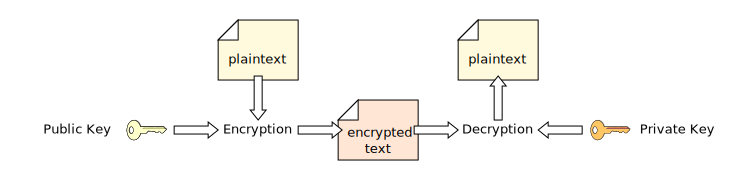
\includegraphics[width=12cm]{tex_tls_echoservice/async2.pdf}}
	\label{fig:asymmetric_encryption}
	\mycaption{specific}{general}
\end{figure}


At startup of the communication process A (Alice) who desires a secure connection transmits her public key to B (Bob).
Bob is now able to encrypt the messages such that only A is able to decrypt them.
As one can see this first approach already provides confidentiality and integrity of messages.
%
Non-repudiation, authentication and due to that access control are not given because the identity of Alice is not proven.
In order to be able to check identities so called certificates must be introduced.
Certificates render the possibility to validate the identity of its owner. They are signed by a certificate authority (CA) which's identity can be resolved to another CA or which is  pre-configured to be trusted.
A certificate is composed of its owner's public key, his identity, the name of the signing CA and a signiture which is a hash-value of the certificate encrypted with the private key of the CA. 
If a certificate can be resolved to a CA with is pre-configured to be trusted, the identity of the certificate owner is considered as to be proven. 
In general a set of trusted CAs is already defined in the operation system.
To obtain a certificate a certificate request has to be submitted to a CA.
After the CA has verified the identity of the requesting person and the requested certificate will be signed.
Figure~\ref{fig:certificate_request} shows the procedure of gaining a certificate.
\begin{figure}[htb]
	\centering%epstopdf certificates.eps
 	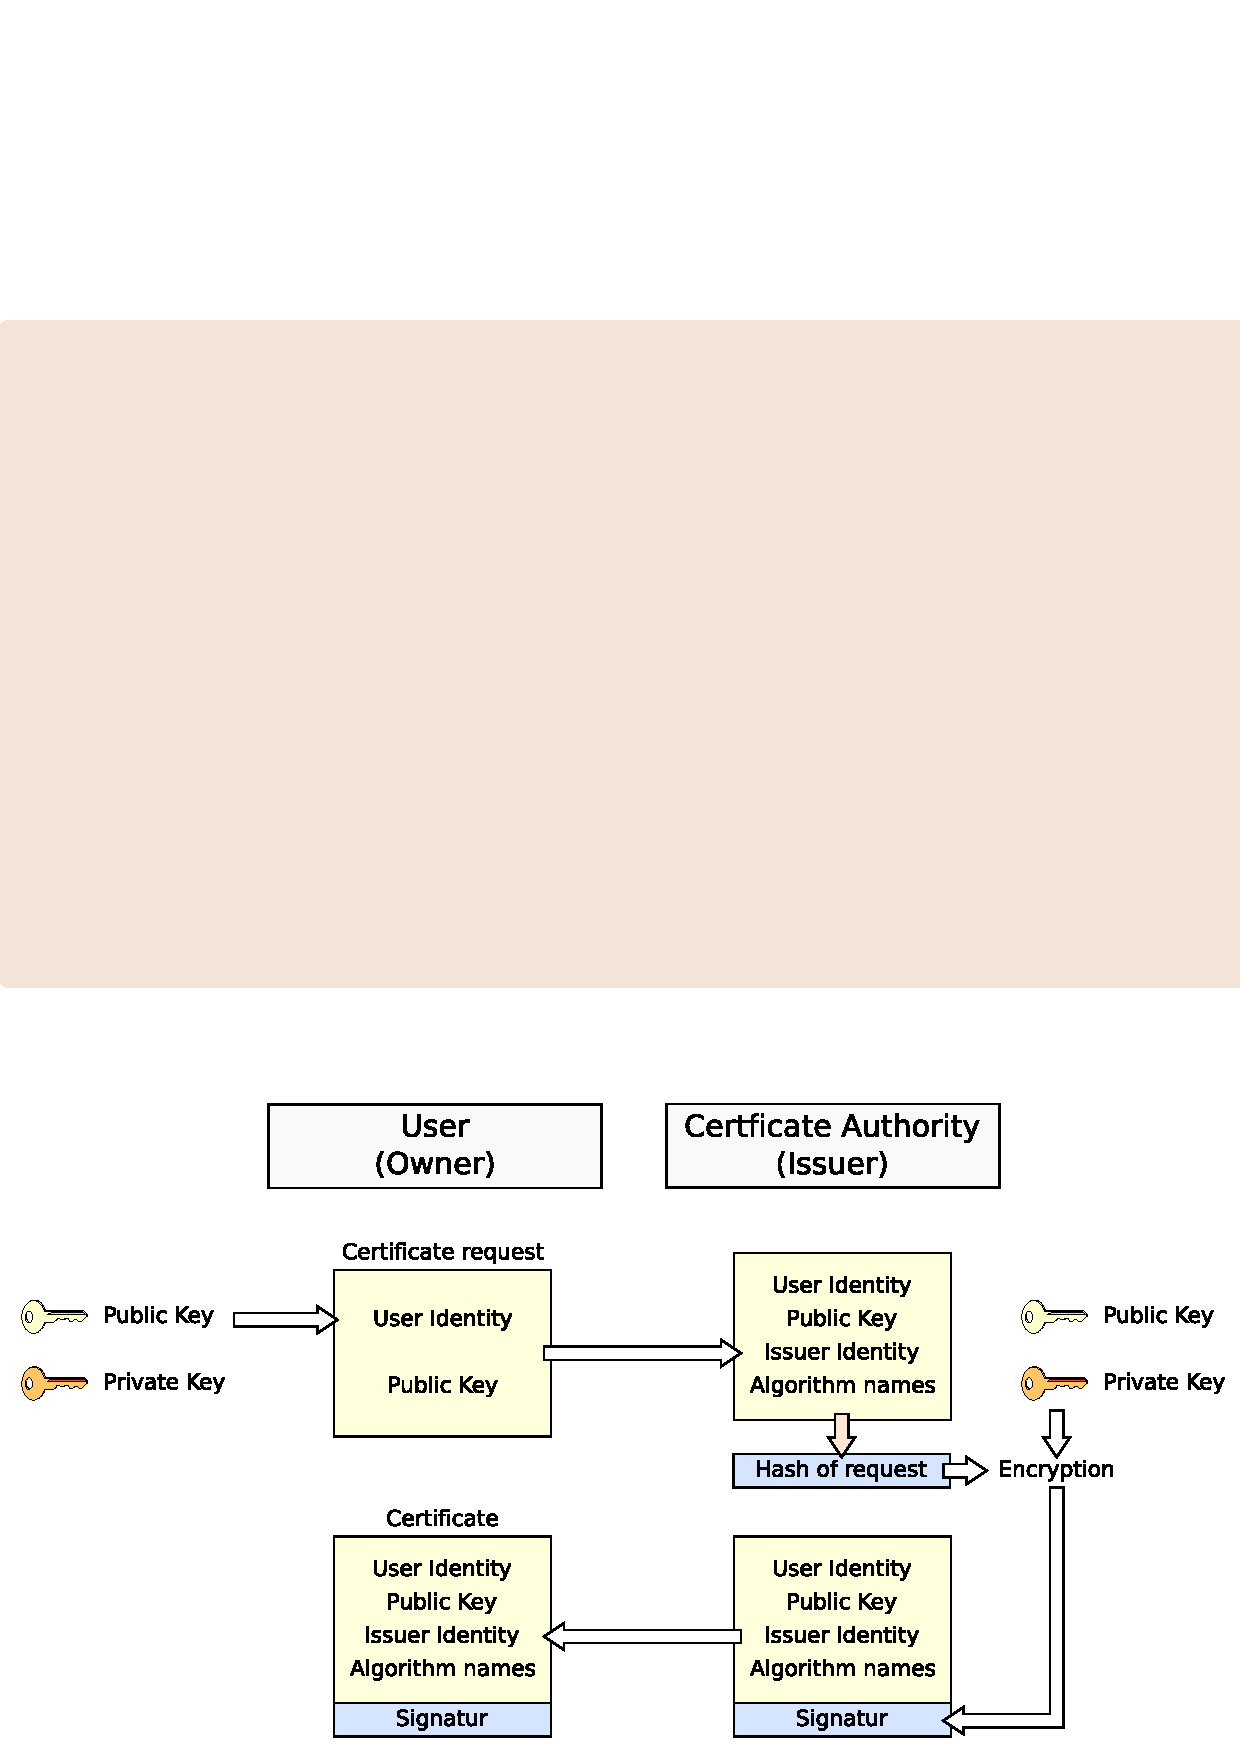
\includegraphics[width=13cm]{tex_tls_echoservice/certificates.pdf}
	\mycaption{specific}{general}
	\label{fig:certificate_request}
\end{figure}
In the first step, a private and a public key will be generated by the requester. The public key together with a textual description of the identity  depict the request which will be transmitted to a CA. After the CA successfully varified the validity of the request, the identity of the CA and the name of used the encryption algorithms are added.
The collected data will represent the plain text of the certificate. In order to ensure the integrity of the text, 
a hash value will be created. (A fixed-sized short string which is generated by an algorithm based on an arbitrary long given text. The algorithm is designed such that a small change in the text will cause the hash value to change almost like a random function. Thus, the hash value can be used a fingerprint of the text.) The CA signs the plain certificate by encrypting its hash value with its private key. Finally the signed certifcate will be returned to the requester.
%
%
If an outside person wants to verify the certificate owner, the encrypted hash value has to be decrypted by the public key of the CA and a hash value has to be created with the same algorithm in order to compare them.\\


Figure~\ref{fig:verification_of_certificates} shows a usecase in which Alice wants to resolve the identity of Bob. Alice submitts her request to Bob along with a challange consisting of a random number $n$. 
The random number ensures that it is not possible to repeat a message (integrity).
Bob encrypts the number with his private key and returns it together with his certificate. Alice uses the public key of Bob to decrypt the challange. 
If the decrypted number is equal to the transmitted number, Alice can reason that the identity of Bob is to be trusted in case she is trusting the CA which has signed Bobs certificate. 
%
In the given example Alice only trusts the CA 2 but not CA 1.
In order to resolve the identity, Alice establishes a connection to CA 1 and submits another random number $n$ as a challenge.
The CA 1 encrypts the challange with its private key and send the result along with its certificate back to Alice. Alice succefully validates the certificate of CA 1. Due to the certificate was signed by CA 2 which is pre-configured to be trusted she can follow to trust CA 1 and in conclusion the identity of B. In summary, Alice knows she is talking to Bob. If Bob also wants to be sure how he's talking to the same procedure has to be done for the identity of Alice. The TLS mode in in which both endpoints are ensuring themself to whom they are talking to is called bilateral connection.
Due to the client is aware of the service authentity, the confidential treatment of his data is given such that it won't be revealed to a third party (service sided confidentiality). Moreover the access to the service can be controled (access control) and the results are only passed back to the right person (client sided confidentiality). 
As one can see confidentiality, authentication, integrity and non-repudiation are now given.\\
\begin{figure}[htb]
	\centering%epstopdf verification.eps 
	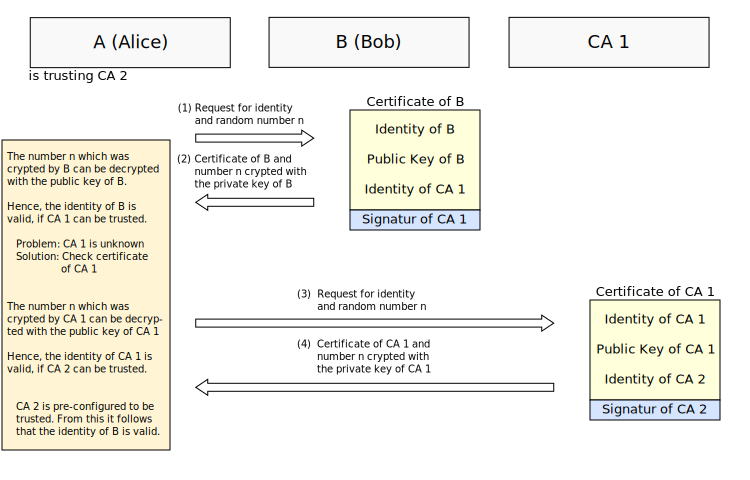
\includegraphics[width=13cm]{tex_tls_echoservice/verification.pdf}
	\mycaption{specific}{general}
	\label{fig:verification_of_certificates}
\end{figure}



Certificates have several advantages. They are scaling very good with the amount of users because CAs can create new sub-CAs such that the load is balanced (certificates of a CA may be cached). Furthermore no critical information is exchanged which may gets intercepted - in particular no secret key is shared. Instead a set of pre-configured CAs which will be in general provided by the operation system is needed.
In respect of ARC it is obvious, that the access to the grid should be under control of its administrator. To do so, the administrator have to build up his own CA to be in charge of creating certificates for a set of users. 
The created CA have to be shipped into the directory of pre-configured CAs.
(Within the source code there are two shell scripts to create a CA and related certificates). Due to there's a bunch of tools for certificates (like \textit{openssl}) it is easy to maintain them. 


o Infrastructure is given and easily to maintain

o In general the pre-configured organistion take money to sign certifcates, but they can also be created locally.

o VOMs are realisable

ARC:

TLS also supports the more secure bilateral connection mode (typically used in enterprise applications), in which both ends of the "conversation" can be ensured with whom they are communicating




o What do we need to get a service running

clientCA   - Authority guarantee for identity
clientCERT - Certificate given
clientKEY  - Secret key of the client to read messages, encrypted by the public key in the certificate!

serverCA   - Authority guarantee for cert. CA is known by the server. If not, the encrypted cert can be read be its CA.
serverCERT - Certificate given by the CA. Contains a snippet which can be read by the Public key of the CA.
serverKEY  - Secret key of the client to read messages, encrypted by the public key in the certificate!


Server has got have:
Its  serverCERT serverKEY and some kind of root CA knowing the client
Client has got to have
Its  clientCERT clientKEY and some kind of root CA knowing the server



\task{RENAMING into~ARC service configuration file}
\task{echo service client configuration file}






%The first two goals can be reached by encrypting the channel/connection between client and server. An approach 
%sich bewähren / behaupten
%which stand the test of time is to introduce a TLS (Transport Layer Security) also known as SSL (Secure Sockets Layer).
%Authenticity, Confidentiality, Integrity
%The client wants to reassure himself to send his vulnerable data only to the server who can prove its correct identity.
%Furthermore a prove of authenticity is needed. % Sich versichern, dass das Gegenüber der ist, für welchen er sich ausgibt
%It .... does fancy stuff ...
%
%
%Authorization:  The server on the other side takes an interest in limitate its ressources to a close circle of users. Above all no %foreign clients shall be able to use the services.\\


\clearpage
\section{Service}

One can add the TLS in client and server by simply extending the arched configuration file and a small modification of the client.



WARNING: If the programm fails, check if one of your certifacte is expired. If so, create new one using the script files in the directory 'certFactory'

For HED is build up to  % entsrprechend einer Mod Structur
be modular, the security can easily be extend to our given example.
Each Message Chain Component (MCC) or service has a common interface for implementing various pluggable components (plug-ins) called SecHandler. The SecHandler components provide a method for processing messages traveling through Message Chains of the HED. 
Each MCC or Service usually implement two queues of SecHandlers – one for incoming messages and one for outgoing called “incoming” and “outgoing” respectively. All SecHandler components attached to the queue are executed sequentially. 
If any of them fails, message processing fails as well. 
Each SecHandler is configured inside the arched configuration file used for configuring whole chain of MCCs 
Some of the currently implemented SecHandler components make use of pluggable and configurable sub-modules called Policy Decision Point (PDP). PDP can process ARC specific Request and Policy documents which are as well written in XML format~\cite{QIANG_2008}..




4 types:
                <KeyPath>./clientKey.pem</KeyPath>
                <CertificatePath>./clientCert.pem</CertificatePath>
                <CACertificatePath>./serviceCA.pem</CACertificatePath>

\lstsetCPP
\lstinputlisting
	[
	label=lst:tls_echo_service_cpp,
	caption={[HED configuration file for the Arc intern echo service. Filename: arcecho\_no\_ssl.xml]
	\textbf{HED configuration file for the Arc intern echo service. Filename: arcecho\_no\_ssl.xml\textcolor{white}{hmf}}}
	]
{../src/services/tlsechoservice/tlsechoservice.cpp}




\lstsetARCHEDXML
\lstinputlisting
	[
	label=lst:tls_echo_arched_xml,float=htb,
	caption={[HED configuration file for the Arc intern echo service. Filename: arcecho\_no\_ssl.xml]
	\textbf{HED configuration file for the Arc intern echo service. Filename: arcecho\_no\_ssl.xml\textcolor{white}{hmf}}}
	]
{../src/services/tlsechoservice/arched_tls_echoservice.xml}


\lstsetKSH
\begin{lstlisting}[
label=lst:tls_echo_arched_invoke,float=htb,
caption={[Transformation in eine uniforme konzentrische Verteilung.]
         \textbf{Transformation in eine uniforme konzentrische Verteilung.\textcolor{white}{hmf}}}]
$ rm -f /var/log/arched.log
$ arched -c arched_echoservice.xml  && echo jo ||echo n
$ tail -n100 -f /var/log/arched.log
$ killall arched
\end{lstlisting}




\clearpage
\section{Client}

\lstsetCPP
\lstinputlisting
	[
	label=lst:tls_echo_client_cpp,
	caption={[HEC configuration file]
	\textbf{HEC configuration file\textcolor{white}{hmf}}}
	]
{../src/clients/tlsechoclient/tlsechoclient.cpp}



Folgender XML Aufruf und Antwort soll \textit{automatisch} generiert werden:

%[caption={[]WegDamit},language=XML,basicstyle=\scriptsize,breaklines=true,label=lst:request] 





Zertifikate
Zustände (Nutzer wiedererkennen, arbeit aufnehmen)




\lstsetKSH
\begin{lstlisting}[
label=lst:tls_echo_client_invoke,float=htb,
caption={[Transformation in eine uniforme konzentrische Verteilung.]
         \textbf{Transformation in eine uniforme konzentrische Verteilung.\textcolor{white}{hmf}}}]
$ ./echoclient
Tue Feb 17 17:04:08 2009
\end{lstlisting}






\lstsetJUSTXML
\begin{lstlisting}[
label=lst:tls_echo_request_XML,float=htb,
caption={[Transformation in eine uniforme konzentrische Verteilung.]
         \textbf{Transformation in eine uniforme konzentrische Verteilung.\textcolor{white}{hmf}}}]
<soap-env:Envelope xmlns:tlsecho="urn:tlsecho" xmlns:soap-enc="http://schemas.xmlsoap.org/soap/encoding/" xmlns:soap-env="http://schemas.xmlsoap.org/soap/envelope/" xmlns:xsd="http://www.w3.org/2001/XMLSchema" xmlns:xsi="http://www.w3.org/2001/XMLSchema-instance">
  <soap-env:Body>
    <tlsecho:tlsechoRequest>
      <tlsecho:say operation="ordinary">text_to_be_transmitted</tlsecho:say>
    </tlsecho:tlsechoRequest>
  </soap-env:Body>
</soap-env:Envelope>
\end{lstlisting}






\lstsetJUSTXML
\begin{lstlisting}[
label=lst:tls_echo_response_XML,float=htb,
caption={[Transformation in eine uniforme konzentrische Verteilung.]
         \textbf{Transformation in eine uniforme konzentrische Verteilung.\textcolor{white}{hmf}}}]
<soap-env:Envelope xmlns:tlsecho="urn:tlsecho" xmlns:soap-enc="http://schemas.xmlsoap.org/soap/encoding/" xmlns:soap-env="http://schemas.xmlsoap.org/soap/envelope/" xmlns:xsd="http://www.w3.org/2001/XMLSchema" xmlns:xsi="http://www.w3.org/2001/XMLSchema-instance">
  <soap-env:Body>
    <tlsecho:tlsechoResponse>
      <tlsecho:hear>[ text_to_be_transmitted ]</tlsecho:hear>
    </tlsecho:tlsechoResponse>
  </soap-env:Body>
</soap-env:Envelope>
\end{lstlisting}


\chapter{Secure Echo Web Service}

The TLS Echo Web Service, which was presented in the previous chapter, was able to control the access to the HED on a very low layer. 
For the administration of a large VO the kind of security may be too general.
Thus, it is recommended to have a more fine grained security. 
This chapter will discuss how to install a more complex security such that it is possible to limitate the access of certain resources to particular users and to narrow their rights on the workstation.\\


The security framework of ARC is implemented based on the same concept of modularity as HED. 
To extend the security of a MCC or a service one only has to modify the server configuration file. That is done by including a \textit{SecHandler} element into the component or service which again has to contain a PDP element. A small example of a chain component containing a \textit{SecHandler} is shown in Listing~\ref{lst:sec_service_component_xml}. Within the element \textit{Component}, which realises a HTTP layer, an element \textit{SecHandler} is located. It contains three attributes. The  attribute \textit{name} is \textit{arc.authz}, the \textit{event} attribute is \textit{incoming} and the \textit{id} attribute which is \textit{auth}. 
While \textit{id} is only an optional parameter, the attribute \textit{name} causes a certain \textit{SecHandler} to be loaded.%, which again has a certain functionality. 
In case the attribute \textit{name} is assigned to \textit{arc.authz}, the SecHandler provides the functionality of authentication and is able to permit or to deny the access to the next layer. 
Each MCC or Service usually implements two queues of \textit{SecHandlers} --- one for incoming messages and one for outgoing messages. The attribute \textit{event} attaches the present one to the incoming queue. \textit{SecHandlers} are able to intervene the message flow by: manipulating the message content, manipulating the message attributes or to disrupt messages.
Within one component, \textit{SecHandlers} are executed sequentially in the order in which they were attached to the queue. If any of them fails, message processing fails as well~\cite{QIANG_2008}. In order to decide how the \textit{SecHandler} shall modify the message so called PDP (Policy Decision Point) are used. Within the example a PDP named \textit{simplelist.pdp} is inserted within the \textit{SecHandler} element. The mechanism of this PDP uses a file which contains a list of identities. If the current identity is on the list, the PDP returns a positive result to the \textit{SecHandler}. In general more than one PDP can be defined within one \textit{SecHandler}. The default behaviour in that case is to execute all PDPs sequentially until one fails such that a negativ result will be returned or all return a negativ result such that also a positive result will be passed to the \textit{SecHandler}.\\
%
%
% Weizhong: Verifying, parsing the message attribute, and using the attributes for authorization
%
% Attributes done by: identity.map, delegation.collector
% manipulating content: usernametoken.handler
% disrupt by: arc.authz
\lstsetJUSTXML
\begin{lstlisting}[
label=lst:sec_service_component_xml,float=htb,
caption={[Example of a SecHandler within the component \textit{http.service}.]
         \textbf{Example of a SecHandler within the component \textit{http.service}}}]
<Component name="http.service" id="http">
	<next id="soap">POST</next>
	<SecHandler name="arc.authz" event="incoming" id="auth">
		<PDP name="simplelist.pdp" location="./clientlist.txt"/>
	</SecHandler>
</Component>
\end{lstlisting}




  \begin{table}[htb]
  \centering
  \caption{List of buildin SecHandlers}
  \label{tbl:list_of_sechandler}
  \begin{tabular*}{\textwidth}[t]{p{4cm}p{11cm}}
	\hline
 	\textbf{identity.map}         & Maps the identity of the user to an identity of the workstation.\\
%					realised by a message attribut.\\
 	\textbf{arc.authz}            & Grants the access to the next layer.\\
 	\textbf{delegation.collector} & Processes a request for another service located on a different HED.
                                        A certificate, which has a delegation policy embedded, is transfered to the service running that \textit{SecHandler}. Once the has been extracted and verified it will be transfered
                                        to the requested service.
                                        The policy is now available within the HED of the service such that the client is now able to access the service.\\
                                        % Question how does the client creates the request - with the SecHandler?
 	\textbf{usernametoken.handler}& Generates the WS-Security username-token and adds it into the SOAP header of outgoing
					 messages. In case of incoming messages the SecHandler extracts the WS-Security username-token out of it. The WS-Security standard extends SOAP and describes i.e. how to attach signatures and encryption header to SOAP messages.\\
	\hline
  \end{tabular*}
  \end{table}
% WS-Security describes how to attach signatures and encryption headers to SOAP messages. In addition, it describes how to attach security tokens, including binary security tokens such as X.509 certificates and Kerberos tickets, to messages.
%
  \begin{table}[htb]
  \centering
  \caption{List of buildin PDPs}
\label{tbl:list_of_pdps}
  \begin{tabular*}{\textwidth}[t]{p{4cm}p{11cm}}
	\hline
 	\textbf{allow.pdp}           & Always returns a positive result.\\
	\textbf{deny.pdp}            & Always returns a negative result.\\
 	\textbf{simplelist.pdp}      & Renders a positive result in case the identity corresponds to the listed ones and additionally 
                                       maps the identity to an user of the workstation.\\
 	\textbf{arc.pdp}             & Evaluates the result based on a policy XML file.\\
 	\textbf{delegate.pdp}        & Similar to \textit{arc.pdp} a policy file will be evaluated. But here, the policy document is 
                                       extracted and transfered
                                       by delegation.collector.\\
 	\textbf{pdpservice.invoker}  & Establishes a connection to special service in order to get a policy decision. The PDP service 
                                       implements the same functionality as ARC PDP, except that the evaluation request and 
                                       response is carried by SOAP messages. The benefit of the PDP Service and the PDP Service
                                       Invoker is that the policy evaluation engine can be accessed remotely and maintained centrally.
\\
	\hline
  \end{tabular*}
  \end{table}
%
%
Due to the fact, that presenting all \textit{SecHandlers} and PDPs would go beyond the scope of an introducing tutorial, only a small set of them will be introduced here in detail. 
Nevertheless, the Tables~\ref{tbl:list_of_sechandler} and~\ref{tbl:list_of_pdps} shall give a first overview about existing \textit{SecHandlers} and \textit{PDPs}. For further reading it is recommended to consult the document ``Security framework of ARC1'' written by Weizhong Qiang and Alexandr Konstantinov. The present chapter is closly related to it.\\


The Secure Echo Web Service which will be presented in this chapter, is using the \textit{SecHandlers}: \textit{indentity.map} and \textit{arc.authz}, and the \textit{PDPs}: \textit{allow.pdp}, \textit{simplelist.pdp} and \textit{arc.pdp}. \\


\section{Service}

Listing~\ref{lst:sececho_service_cpp} contains the source code of the Secure Echo Web Service. As one can see, the only diffrence, compared to the source code of the previous section, is the additional code to process the \textit{SecHandler} starting at line~\ref{lst_code:sececho_service_cpp_process_secH}. Obviously only the incoming queue is processed and in case the SecHandler fails, the SOAP service returns a fault message. The file, which is revealing a lot more information, is the server configuration file which is shown in Listing~\ref{lst:sececho_server_configuration_file_xml}. 
In order to be able to have \textit{SecHandlers} working with identies, it is almost essential to utilise the TLS layer.
% Fixed IP are also possible but not recommended..
The TLS layer extracts the identity such that it later can be used to process the \textit{SecHandler}.
In line~\ref{lst_code:arched_sec_conffile_plugins} and line~\ref{lst_code:arched_sec_conffile_plugins2} two additional plugins 
are named to be loaded which are implementing of the \textit{SecHandlers} and \textit{PDPs}.
%
%  FIRST ONE
%
The first \textit{SecHandler} is declared within line~\ref{lst_code:arched_sec_conffile_secH2}. 
Due to the PDP \textit{allow.pdp} returns always a positive result, everyone who passes the \textit{SecHandler} is mapped to the user \textit{nobody}. 
%
% SECOND ONE
%
The second \textit{SecHandler} limits the access to the SOAP services using the \textit{arc.authz} \textit{SecHandler} and the \textit{simplelist} policy, see line~\ref{lst_code:arched_sec_conffile_secH1}. (A similar example was already shown in Listing~\ref{lst:sec_service_component_xml}). The \textit{simplelist} policy returns a positive result if the identity of the certificate corresponds to an identity within the file \textit{clientlist.txt}. A small example of such a file is displayed in Listing~\ref{lst:simplelist_example}.
\lstsetCPP
\lstinputlisting
	[
	label=lst:sececho_service_cpp,
	caption={[Source code of the Secure Echo Service.]
	\textbf{Source code of the Secure Echo Service.}}
	]
{../src/services/secechoservice/secechoservice.cpp}
%
%
The first part of an entry needs to be the distinguished name (DN) of the current client. A DN is a string which represents a user uniquely and is created using the identity of the certificate. To get the correct DN of a client one can use the TLS Echo Web Service and check the log-file. The second part of an entry specifies the user the identity shall be mapped to. In the present case, the identity will be mapped to \textit{griduser}. In case the policy is unable to match the identity, the PDP returns a negativ result.
The \textit{SecHandler} within the SOAP component limits the access of SOAP to a certain group of users.
%
%
% The third ONE
The last \textit{SecHandler}, used in the server configuration file, is to be seen starting with line~\ref{lst_code:arched_sec_conffile_secH3}. The \textit{SecHandler} is chosen to be \textit{arc.authz} which leads to the fact that the access to the Echo Web Service will be limited one more time to a subset of the group. The policy \textit{arc.pdp} returns a positive result in case the rules encapsulated within the file \textit{policy.xml} will return a positive result.\\
\lstsetARCHEDXML
\lstinputlisting
	[
	label=lst:sececho_server_configuration_file_xml, float=htb
	caption={[HED configuration file for the Arc intern echo service. Filename: arcecho\_no\_ssl.xml]
	\textbf{HED configuration file for the Arc intern echo service. Filename: arcecho\_no\_ssl.xml\textcolor{white}{hmf}}}
	]
{../src/services/secechoservice/arched_sec_echoservice.xml}



\lstsetKSH
\begin{lstlisting}[
label=lst:simplelist_example, float=htb,
caption={[Appearence of the file used by \textit{simplelist.pdp}.]
         \textbf{Appearence of the file used by \textit{simplelist.pdp}.}}]
$ cat clientlist.txt
"/C=US/S=Maine/OU=Literary character/O=Ka-Tet Corp./CN=Roland Deschain" griduser
"/C=US/S=Maine/OU=Literary character/O=Ka-Tet Corp./CN=Susannah Dean" griduser
$
\end{lstlisting}

If the PDP \textit{arc.authz} is used, a bunch of requests will be generated for the client. The requests are compared with the rules defined in the policy and for each rule a decision is made.
A sample policy is shown in Listing~\ref{lst:sececho_policy_xml}. The main element is \textit{policy} which encloses three elements called \textit{Rule}\footnote{The latest XML schema for defining an \textit{arc.pdp} policy can be found at \url{http://svn.nordugrid.org/trac/nordugrid/browser/arc1/trunk/src/hed/shc/arcpdp/Policy.xsd}}. 
Two types of rules are possible: a permitting or a denying rule.
A Rule may have four different decision states:
\begin{itemize}
 \item PERMIT --- A permitting rule returns the decision permit if one request fits to the rule and 
the request is fullfilled by the rule. (A denying rule would return deny in that case)
 \item DENY --- A permitting rule returns the decision deny if one request fits to the rule  and the request is not fullfilled by the rule. (A denying rule would return permit that case)
 \item INDETERMINATE --- Requests and rule have some parts which not fits
(i.e. shibboleth identity is checked, but user has identified himself via X.509 and additionally an existing resource is requested)
 \item NOT\_APPLICABLE --- If the request doesn't fit with the rule at all. (i.e. if the 
request is for the HTTP method GET, but the rule checks the method POST)
\end{itemize}
\forcelinebreak

Once all rules are evaluated, a decision for the policy has to be generated which will depend on the results of the rules.
The policy element attribute \textit{CombiningAlg} determines how the final result will be generated. Two possibility are given:
\begin{itemize}
 \item \textbf{Deny-Overrides} (default) 
 \begin{itemize}
	\item If there is at least one DENY in results final result is DENY. 
	\item Otherwise if there is at least one PERMIT, the final result is PERMIT.
	\item Otherwise if there is at least one NOT\_APPLICABLE final result is NOT\_APPLICABLE.
	\item Otherwise final result is INDETERMINATE.
 \end{itemize}
  \item \textbf{Permit-Overrides}
 \begin{itemize}
 	\item If there is at least one PERMIT in results final result is PERMIT.
 	\item Otherwise if there is at least one DENY the final result is DENY.
 	\item Otherwise if there is at least one NOT\_APPLICABLE final result is NOT\_APPLICABLE.
 	\item Otherwise final result is INDETERMINATE.
 \end{itemize}
\end{itemize}
\forcelinebreak

A rule is devided into four sub-elements: \textit{Subjects}, \textit{Resources}, \textit{Actions} and \textit{Conditions}. 
The element \textit{Subjects} defines who shall be affected by that rule.
The identities can be specified using the DN of the certificate.
The second element determines the \textit{Resources} which shall be examined by the rule (i.e. using a certain HTTP path).
The \textit{Actions} are specifing the intended usage of the resource the rule shall survey.
The last element \textit{Condition} defines somewhat like Time, Duration, namespace of a SOAP message etc. which is needed to be fulfilled.
For the description of conditions is complicated, they will not be explained in this tutorial.\\


Within the sample policy, which was shown in Listing~\ref{lst:sececho_policy_xml}, three different examples of rule states are prepared: PERMIT, INDETERMINATE and NOT APPLICABLE.
The first rule, to be seen starting at line~\ref{lst_code:policy.xml_rule1}, is fitting to the server configuration file such that a user with a suitable identity will produce the state PERMIT. 
Due to there is no rule within the policy which will have the DENY state, this rule let the client pass the PDP.
The second rule, begins after line~\ref{lst_code:policy.xml_rule2}. It is arranged in a manner such that the state INDETERMINATE will be induced. Two things are checked within it: The identity based on Shibboleth authentication and the path of the requested HTTP URL. Due to the fact, that the HTTP path is fitting to the requested one, but the authentication was not done by Shibboleth, the rule is not able to decide for a DENY or a PERMIT state --- the rule produces an INDETERMINATE state.
The last rule is defined in line~\ref{lst_code:policy.xml_rule3}. It is constructed such that is permits the access to the HTTP method GET. 
One can see, that within the server configuration file the Web Service uses the method POST. If a client wants to access the Service and reaches the PDP, a couple of requests are generated which are describing the manner the client wants to access the serivice. Some of these request will concern the HTTP method GET. In these cases, the rule returns NOT APPLICABLE. In the cases where the requests for a HTTP method is missing (i.e. in the request which only concerns the SOAP access) the state of the rule will be INDETERMINATE.\\
\lstsetJUSTXML
\lstinputlisting
	[
	label=lst:sececho_policy_xml, float=htb,
	caption={[Policy file for the \textit{arc.pdp} policy decision point.]
	\textbf{Policy file for the \textit{arc.pdp} policy decision point.}}
	]
{../src/services/secechoservice/policy_example.xml}


To get an impression in how the requests look like, one can check the log-file (the log level needs to set to VERBOSE).


\section{Client}

The security introduced to the server has no effect on the client, such that the source code is absolutly identical. Even the client configuration file doesn't need to be changed.

















 
\chapter{Persistent Webservice}


export ARC\_BARTENDER\_URL


    key\_file = os.environ.get('ARC\_KEY\_FILE', None)
    cert\_file = os.environ.get('ARC\_CERT\_FILE', None)
    proxy\_file = os.environ.get('ARC\_PROXY\_FILE', None)
    ca\_file = os.environ.get('ARC\_CA\_FILE', None)
    ca\_dir = os.environ.get('ARC\_CA\_DIR', None)

export ARC\_KEY\_FILE=/local/glodek/clientKey.pem
export ARC\_CA\_FILE=/local/glodek/clientCA.pem
export ARC\_CERT\_FILE=/local/glodek/clientCert.pem

does the daemon runs the service single threaded

race conditions
\begin{itemize}
 \item Transaktionen
 \item nur lesen
 \item jeder prozess schreibt in seine eigene Datei
 \item Gibt es einen     // andere Zugriffe abblocken
    flock (\$fp, LOCK\_EX);  (atomare befehle)
 	wie bei php??
 \item Peterson Algorithmus
 \item Was passiert beim Ausfall (Time out - Transaktion zurück nehmen)
\end{itemize}


\chapter{Appendix}

\section{More tutorials}

Other tutorials are:\\
\\
%Oxana reported the status of OGF tutorials:
\begin{itemize}
 \item first tutorial will be given by Oxana and will deal with how to add the 
resources to Nordugrid, .... (will be related mostly to production ARC)
 \item second tutorial will be given by Gabor and he will show the 
interoperability of ARC (video demo will be shown). A-REX - Unicore 
interoperability.
 \item there will be also a tutorial related to ETICS system where the 
possibility of ETICS system to submit a job to ARC and Unicore will be 
presented. The ETICS team has not contacted so far.
\end{itemize}


\section{Important XSD files}


Link to current XSD files.

\task{Provide a list of modules to be loaded! Along with the implemented functionality which can be addressed with XML elements!!}
    mcctcp\\
\begin{verbatim}
<tcp:Listen>
	<tcp:Port>60000</tcp:Port>
	<tcp:Version>4</tcp:Version>
</tcp:Listen>
\end{verbatim}
    mcctls\\
\begin{verbatim}
 			<KeyPath>./clientKey.pem</KeyPath>
			<CertificatePath>./clientCert.pem</CertificatePath>
			<CACertificatePath>./clientCA.pem</CACertificatePath><!-- CACertificatesDir Should be /etc/... blub mention that-->

\end{verbatim}

    mcchttp\\
\begin{verbatim}
                      <next id="soap">POST</next>
                      <next id="plexer">GET</next>
                      <next id="plexer">PUT</next>
\end{verbatim}
    mccsoap\\
\begin{verbatim}
	???<ClientSSLConfig FromFile='filename'/>  
\end{verbatim}






\bibliography{literature}
\bibliographystyle{IEEEtran}                       % A nice bibliography style


\end{document}
